% !TEX program = xelatex

\documentclass{article}
\usepackage{amsfonts,amssymb}
\usepackage{amsmath}
\usepackage{amsthm}
\usepackage[left=1.0cm,right=1.0cm,top=1.3cm,bottom=1.3cm]{geometry}
\usepackage{enumerate}
\usepackage{fancyhdr}
\usepackage{ctex}
\usepackage{xpatch}
\usepackage{graphicx} %插入图片的宏包
\usepackage{float} %设置图片浮动位置的宏包
\usepackage{subfigure} %插入多图时用子图显示的宏包
\usepackage{listings}
\usepackage{color}
\usepackage{amssymb,mathrsfs,amsmath}
\usepackage{bbding}

\definecolor{dkgreen}{rgb}{0,0.6,0}
\definecolor{gray}{rgb}{0.5,0.5,0.5}
\definecolor{mauve}{rgb}{0.58,0,0.82}

\lstset{frame=tb,
  language=Python,
  aboveskip=3mm,
  belowskip=3mm,
  showstringspaces=false,
  columns=flexible,
  basicstyle={\small\ttfamily},
  numbers=none,
  numberstyle=\tiny\color{gray},
  keywordstyle=\color{blue},
  commentstyle=\color{dkgreen},
  stringstyle=\color{mauve},
  breaklines=true,
  breakatwhitespace=true,
  tabsize=3
}


\newtheoremstyle{break}
    {\topsep}{\topsep}%
    {\itshape}{}%
    {\bfseries}{}%
    {\newline}{}%
\theoremstyle{break}
\newtheorem*{solution*}{\textbf{Solution:} }
%\newtheorem*{proof*}{\textbf{Proof:}}
\makeatletter

\AtBeginDocument{\xpatchcmd{\@thm}{\thm@headpunct{.}}{\thm@headpunct{}}{}{}}
\makeatother

\pagestyle{fancy} 
\lhead{Name}
\chead{\textbf{Discrete Mathematics:  Homework 8}}
\rhead{2020.4.29}
\renewcommand{\baselinestretch}{1.5}

\title{Discrete Mathematics:  Homework 8}
\author{Name  \quad  \quad ID: Number}
\date{2020.4.29}


\begin{document}
\maketitle
\begin{enumerate}
        \item Let $Z^2= {(a, b) :a, b\in \mathbb{Z}}$.  Define $\bigoplus$ and $\bigotimes$ over $\mathbb{Z}^2$ such that,
        \begin{enumerate}
                \item $(a, b)\bigoplus(c, d) = (a+c, b+d)$ ; and
                \item  $(a, b)\bigotimes(c, d) = (ac, bd)$.
        \end{enumerate}
        for all $(a, b),(c, d)\in \mathbb{Z}^2$.  Prove or disprove that $(\mathbb{Z}^2,\bigoplus,\bigotimes)$ is a ring.
        \begin{proof}
                \leavevmode\\
                \begin{enumerate}
                        \item Proof $(\mathbb{Z}^2,\bigoplus)$ is an Abelian group.
                        \begin{enumerate}
                                \item Closure: $\forall (a,b) , (c,d)\in \mathbb{Z}^2, (a, b)\bigoplus(c, d) = (a+c, b+d) \in \mathbb{Z}^2$
                                \item Asssociative: $\forall (a,b) , (c,d), (e,f)\in \mathbb{Z}^2$, \\$((a, b)\bigoplus(c, d) )\bigoplus (e,f)=(a+c, b+d) \bigoplus (e,f) = (a+c+e, b+d+f) = (a,b) \bigoplus (c+e, d+f)=(a, b)\bigoplus((c, d) \bigoplus (e,f))$
                                \item Identity: $\exists (0,0) \in \mathbb{Z}^2, \forall (a,b) \in \mathbb{Z}^2, (a,b)\bigoplus(0,0) = (a,b) = (0,0) \bigoplus (a,b)$
                                \item Inverse: $\forall (a,b) \in \mathbb{Z}^2, \exists(-a,-b) \in \mathbb{Z}^2, (a,b) \bigoplus (-a,-b) = (0,0)$
                        \end{enumerate}
                        \item Proof $(\mathbb{Z}^2,\bigotimes)$ satisfies the property of closure and asssociativity
                        \begin{enumerate}
                                \item Closure: $\forall (a, b),(c, d)\in \mathbb{Z}^2$,$(a, b)\bigotimes(c, d) = (ac, bd) \in \mathbb{Z}^2$
                                \item Asssociativity: $\forall (a,b) , (c,d), (e,f)\in \mathbb{Z}^2$, \\ $((a, b)\bigotimes(c, d) )\bigotimes (e,f)=(ac, bd) \bigotimes (e,f) = (ace, bdf) = (a,b) \bigotimes (ce, df)=(a, b)\bigotimes((c, d) \bigotimes (e,f))$
                        \end{enumerate}
                        \item Distributive Law: 
                        \begin{enumerate}
                                \item $\forall (a,b),(c,d),(e,f) \in \mathbb{Z}^2$, \\$(a,b) \bigotimes ((c,d) \bigoplus (e,f)) = (a,b) \bigotimes (c+e, d+f) = (ac +ae, bd+bf) \\= (ac,bd) \bigoplus (ae,bf) = ((a,b)\bigotimes(c,d) ) \bigoplus ((a,b) \bigotimes (e,f))$
                                \item $\forall (a,b),(c,d),(e,f) \in \mathbb{Z}^2$, \\ we have $((a,b)\bigoplus(c,d))\bigotimes(e,f) = ((a,b)\bigotimes(e,f) )\bigoplus ((c,d)\bigotimes (e,f))$\\
                                The proof is similiar
                        \end{enumerate}
                \end{enumerate}
        \end{proof}
        \newpage
        \item Let $\mathbb{Z}[X]  =\{f_0+f_1X+\dots+f_dX^d :d\geq 0, f_0, f_1, \dots , f_d \in \mathbb{Z}\}$ be  the  set  of  allpolynomials over $\mathbb{Z}$.  Prove or disprove that $(\mathbb{Z}[X],+,·)$ is a ring, where $+$ and $·$ are the additionand the multiplication of polynomials over $\mathbb{Z}$.
        \begin{proof}
                \leavevmode\\
                \begin{enumerate}
                        \item Prove $(\mathbb{Z}[X], +)$ is an Abelian group.
                        \begin{enumerate}
                                \item Closure: \\
                                Let $A \in \mathbb{Z}[X]  =\{f_0+f_1X+\dots+f_dX^d :d\geq 0, f_0, f_1, \dots , f_d \in \mathbb{Z}\}$\\
                                Let $B \in \mathbb{Z}[X]  =\{g_0+g_1X+\dots+g_eX^e :e\geq 0, g_0, g_1, \dots , g_e \in \mathbb{Z}\}$\\
                                W.L.O.G, Suppose $e >f$\\
                                $A+B= \{(f_0+g_0)+(f_1+g_1)X+\dots+(f_d+g_d)X^d + \dots +  g_eX^e\} \in \mathbb{Z}[X]$
                                \item Asssociative:\\
                                W.L.O.G, Suppose $f < g < e$\\
                                Let $A \in \mathbb{Z}[X]  =\{f_0+f_1X+\dots+f_dX^d :d\geq 0, f_0, f_1, \dots , f_d \in \mathbb{Z}\}$\\
                                Let $B \in \mathbb{Z}[X]  =\{g_0+g_1X+\dots+g_eX^e :e\geq 0, g_0, g_1, \dots , g_e \in \mathbb{Z}\}$\\
                                Let $C \in \mathbb{Z}[X]  =\{h_0+h_1X+\dots+h_iX^i :i\geq 0, h_0, h_1, \dots , h_i \in \mathbb{Z}\}$\\
                                $(A+B)+C=(f_0+g_0)+(f_1+g_1)X+\dots+(f_d+g_d)X^d + \dots +  g_eX^e + h_0+h_1X+\dots+h_iX^i  = (f_0 + g_0 + h_0) + (f_1+g_1+h_1)X + \dots + (f_d+g_d+h_d)X^d + \dots (g_e + h_e)X^e + \dots h_iX^i$ \\
                                $A+(B+C) = f_0+f_1X+\dots+f_dX^d + ((g_0 + h_0) + (g_1 + h_1)X + \dots + (g_e + h_e)X^e + \dots h_iX^i) = (f_0 + g_0 + h_0) + (f_1+g_1+h_1)X + \dots + (f_d+g_d+h_d)X^d + \dots (g_e + h_e)X^e + \dots h_iX^i$
                                \item Identity: \\
                                $\exists I = \{0 + 0 +\dots + 0\} \in \mathbb{Z}[X], \forall A \in \mathbb{Z}[X], A+I = A$
                                \item Inverse: 
                                $\forall A \in \mathbb{Z}[X] \exists -A \in \mathbb{Z}[X] $, such that $A + (-A) = I$ 
                        \end{enumerate}
                        \item Proof $(\mathbb{Z}[X], ·)$ satisfies the property of closure and asssociativity
                        \begin{enumerate}
                                \item Closure\\
                                Let $A \in \mathbb{Z}[X]  =\{f_0+f_1X+\dots+f_dX^d :d\geq 0, f_0, f_1, \dots , f_d \in \mathbb{Z}\}$\\
                                Let $B \in \mathbb{Z}[X]  =\{g_0+g_1X+\dots+g_eX^e :e\geq 0, g_0, g_1, \dots , g_e \in \mathbb{Z}\}$\\
                                W.L.O.G, Suppose $e >f$\\
                                $A \cdot B = (f_0 \cdot g_0) + (f_1g_0 +  f_0g_1) X \dots (f_dg_e)X^{d+e} \in \mathbb{Z}[X] $
                                \item Asssociativity
                                W.L.O.G, Suppose $f < g < e$\\
                                Let $A \in \mathbb{Z}[X]  =\{f_0+f_1X+\dots+f_dX^d :d\geq 0, f_0, f_1, \dots , f_d \in \mathbb{Z}\}$\\
                                Let $B \in \mathbb{Z}[X]  =\{g_0+g_1X+\dots+g_eX^e :e\geq 0, g_0, g_1, \dots , g_e \in \mathbb{Z}\}$\\
                                Let $C \in \mathbb{Z}[X]  =\{h_0+h_1X+\dots+h_iX^i :i\geq 0, h_0, h_1, \dots , h_i \in \mathbb{Z}\}$\\
                                $(A \cdot B) \cdot C = ((f_0 \cdot g_0) + (f_1g_0 +  f_0g_1) X \dots (f_dg_e)X^{d+e} )\cdot C = (f_0 \cdot g_0 \cdot h_0) + \dots + (f_d \cdot g_e \cdot h_i) X^{d+e+i}$\\
                                Similiarly, we can prove $(A \cdot B) \cdot C  = A \cdot (B \cdot C)$
                        \end{enumerate}
                        \item Distributive Law: 
                        W.L.O.G, Suppose $f < g < e$\\
                        Let $A \in \mathbb{Z}[X]  =\{f_0+f_1X+\dots+f_dX^d :d\geq 0, f_0, f_1, \dots , f_d \in \mathbb{Z}\}$\\
                        Let $B \in \mathbb{Z}[X]  =\{g_0+g_1X+\dots+g_eX^e :e\geq 0, g_0, g_1, \dots , g_e \in \mathbb{Z}\}$\\
                        Let $C \in \mathbb{Z}[X]  =\{h_0+h_1X+\dots+h_iX^i :i\geq 0, h_0, h_1, \dots , h_i \in \mathbb{Z}\}$\\
                        $A \cdot (B+C) = A \cdot (\sum_{m=0}^{e}X^m + \sum_{n=e+1}^{i}X^n) = f_0g_0h_0 + \dots + f_dh_iX^{d+f}$\\
                        $ab + ac = _0g_0h_0 + \dots + f_dh_iX^{d+f}$  \\
                        Similiarly, $(A+B)\cdot C = ac + bc$
                \end{enumerate}
        \end{proof}
        \vspace{20mm}
        \item Write a computer program to reconstruct the secret $s \in \mathbb{Z}_{1125899906900597}$ in Shamir's $(5,9)-threshold$ secret sharing scheme.  In the devised program, the reconstruction of $s$ shouldbe based on the Lagrange interpolation formula.  Use your program to reconstruct the secret $s$, given that the $9$ shares are as follows:
        \begin{center}
                \begin{tabular}{|c|c|}
                        \hline
                        $i$ & $s_i$ \\
                        \hline
                        1 & 75044643784737 \\
                        \hline
                        2 & 940519894412855 \\
                        \hline
                        3 & 941263003333598 \\
                        \hline
                        4 & 736739711411826 \\
                        \hline
                        5 & 254180887785524 \\
                        \hline
                        6 & 940382343666996 \\
                        \hline
                        7 & 132205297839880 \\
                        \hline
                        8 & 63775631863924 \\
                        \hline
                        9 & 1111084448671404 \\
                        \hline
                \end{tabular}
        \end{center}
        \vspace{10mm}
        \begin{solution*}
                The Code is as follows,\\
                \begin{lstlisting}

                        import collections
                        import sys
                        sys.setrecursionlimit(10000000) #Enlarge maximum recursion depth 
                        
                        def Exgcd(a: int, b: int):
                            '''
                                    gcd(a,b)=ax+by
                            '''
                            if (not b):
                                return [1, 0]
                            x, y = Exgcd(b, a % b)
                            return [y, x - a // b * y]
                        
                        def inv(x: int, mod: int):
                                return Exgcd(x, mod)[0] % mod
                        
                        def TSSS(mod: int, **args) -> int:
                                '''
                                args: dic{}
                        
                                return secret s = f(0) by Lagrange Interpolation
                                '''
                                s = 0
                                for i in args:
                                        terms = 1 #Terms of each f(i)delta_i(0)
                                        deno = 1  #Denominator
                                        for j in args:
                                                if i == j:
                                                        continue
                                                terms = terms * (0 - int(j))
                                                deno = deno * (int(i) -int(j))
                                        s += args[i] * terms * inv(deno, mod)
                                        s %= mod
                                return s
                        
                        d = {
                            '1': 75044643784737,
                            '2': 940519894412855,
                            '3': 941263003333598,
                            '4': 736739711411826,
                            '5': 254180887785524
                        }
                        
                        print(TSSS(1125899906900597, **d))                                           
                \end{lstlisting}
        And the Output is : 
        \[
                330836359559300
        \]
        \end{solution*}
        \newpage
        \item  An  officer  stored  in  his  safe  a  very  important  letter.    He  shared  the  password $s \in \mathbb{Z}_{1125899906900597}$ to  the  safe  among  $9$  soldiers  using  $Shamir’s  (5,9)-threshold$  secret  shar-ing scheme.  After the officer was killed in a battle, the $9$ soldiers need to open the safe.  Supposethat they provided the following shares in the reconstruction process:
        \begin{center}
                \begin{tabular}{|c|c|}
                        \hline
                        $i$ & $s_i$ \\
                        \hline
                        1 &  150550125355646 \\
                        \hline
                        2 &    944474507418938 \\
                        \hline
                        3 & 110040335185999 \\
                        \hline
                        4 & 676042268761809 \\
                        \hline
                        5 & 193274108888331 \\
                        \hline
                        6 & 904128547609081 \\
                        \hline
                        7 & 354197665334455 \\
                        \hline
                        8 & 416432161112962 \\
                        \hline
                        9 & 283942097426448 \\
                        \hline
                \end{tabular}
        \end{center}
        Among  the  9  soldiers  2  were  spies  and  provided  wrong  shares  in  order  to  prevent  the  othersoldiers from opening the safe.  Use your computer program in Question 3 to find the spies andthen recover the password $s$ from the correct shares。
        \vspace{10mm}
        \begin{solution*}
               The Code is as follows:\\
                \begin{lstlisting}
                        import collections
                        import sys
                        from itertools import combinations, permutations
                        sys.setrecursionlimit(10000000) #Enlarge maximum recursion depth 
                        
                        def Exgcd(a: int, b: int):
                            '''
                                    gcd(a,b)=ax+by
                            '''
                            if (not b):
                                return [1, 0]
                            x, y = Exgcd(b, a % b)
                            return [y, x - a // b * y]
                        
                        def inv(x: int, mod: int):
                                return Exgcd(x, mod)[0] % mod
                        
                        def TSSS(mod: int, **args) -> int:
                                '''
                                args: dic{}
                        
                                return secret s = f(0) by Lagrange Interpolation
                                '''
                                s = 0
                                for i in args:
                                        terms = 1 #Terms of each f(i)delta_i(0)
                                        deno = 1  #Denominator
                                        for j in args:
                                                if i == j:
                                                        continue
                                                terms = terms * (0 - int(j))
                                                deno = deno * (int(i) -int(j))
                                        s += args[i] * terms * inv(deno, mod)
                                        s %= mod
                                return s
                        
                        def remove(list:list, element):
                                for i in list:
                                        if i == element:
                                                list.remove(i)
                        
                        
                        d = {
                            '1': 150550125355646,
                            '2': 944474507418938,
                            '3': 110040335185999,
                            '4': 676042268761809,
                            '5': 193274108888331,
                            '6': 904128547609081,
                            '7': 354197665334455,
                            '8': 416432161112962,
                            '9': 283942097426448
                        }
                        
                        
                        C = list(combinations([1, 2, 3, 4, 5, 6, 7, 8, 9], 5))
                        num = [1,2,3,4,5,6,7,8,9]
                        list = list()
                        for i in C:
                                dic = dict()
                                for j in range(5):
                                        dic[str(i[j])] = d[str(i[j])]
                                print(i)
                                print(TSSS(1125899906900597, **dic))
                                list.append(TSSS(1125899906900597, **dic))
                                print()
                                if (TSSS(1125899906900597, **dic) == 516971327093293):
                                        for j in range(5):
                                                remove(num,i[j])
                        print(num)
                        
                        # print(list)
                        # dict_num = {}
                        # for item in list:
                        #     if item not in dict_num.keys():
                        #         dict_num[item] = list.count(item)
                        
                        # import operator
                        # sorted(dict_num.items(),key=operator.itemgetter(1))
                        
                        # print (dict_num)
                \end{lstlisting}
                The Output:
                \begin{figure}[H]
                        \centering
                        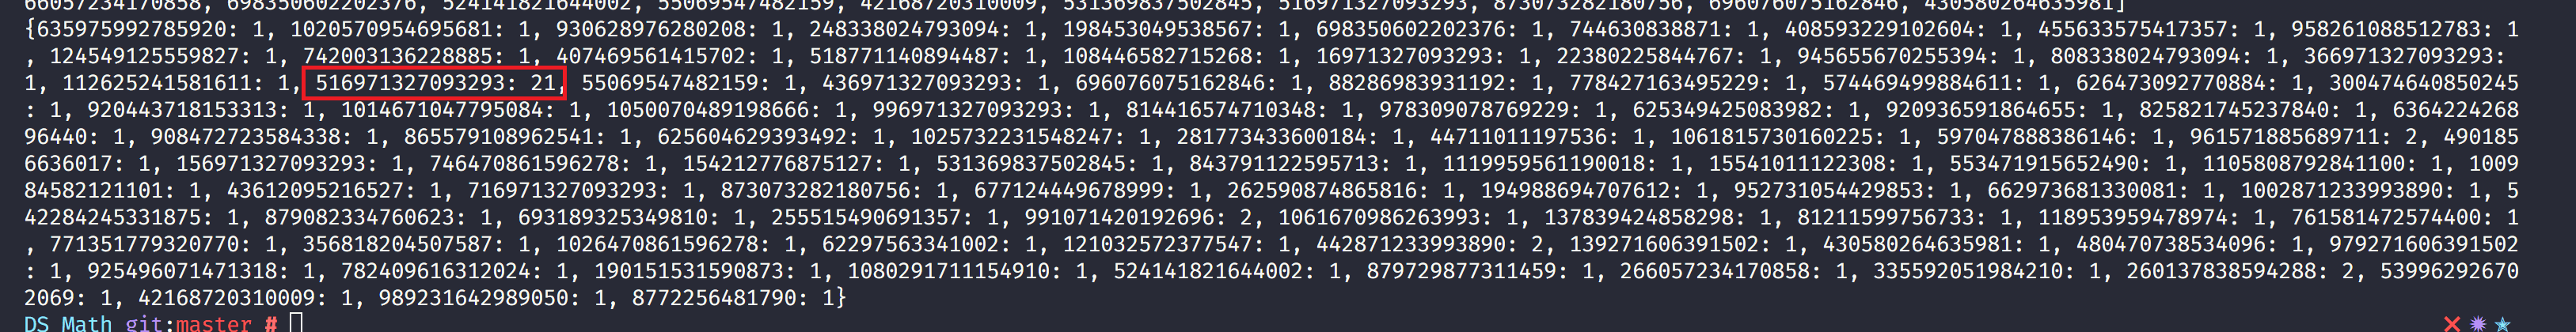
\includegraphics[scale=0.36]{2.png}
                \end{figure}
                and,
                \[      
                        [3, 7]
                \]
                First we find $s = 516971327093293$ , because it is the most seen number in the list of results.\\
                Than we find spi is $3,7$ because everytime when the answer is correct, $3,7$ doesn't take any part.
        \end{solution*}
        \vspace{20mm}
        \item Let $=\{P1, P2, P3, P4, P5\}$.  Design a secret sharing scheme that realizes an accessstructure with basis
        \[
                \tau_0=\{\{P_1, P_2\},\{P_1, P_3\},\{P_1, P_4, P_5\,\{P_2, P_3, P_4\},\{P_2, P_3, P_5\},\{P_2, P_4, P_5\},\{P_3, P_4, P_5\}\}.
        \]
        \begin{solution*}
                \leavevmode\\
                \begin{figure}[H]
                        \centering
                        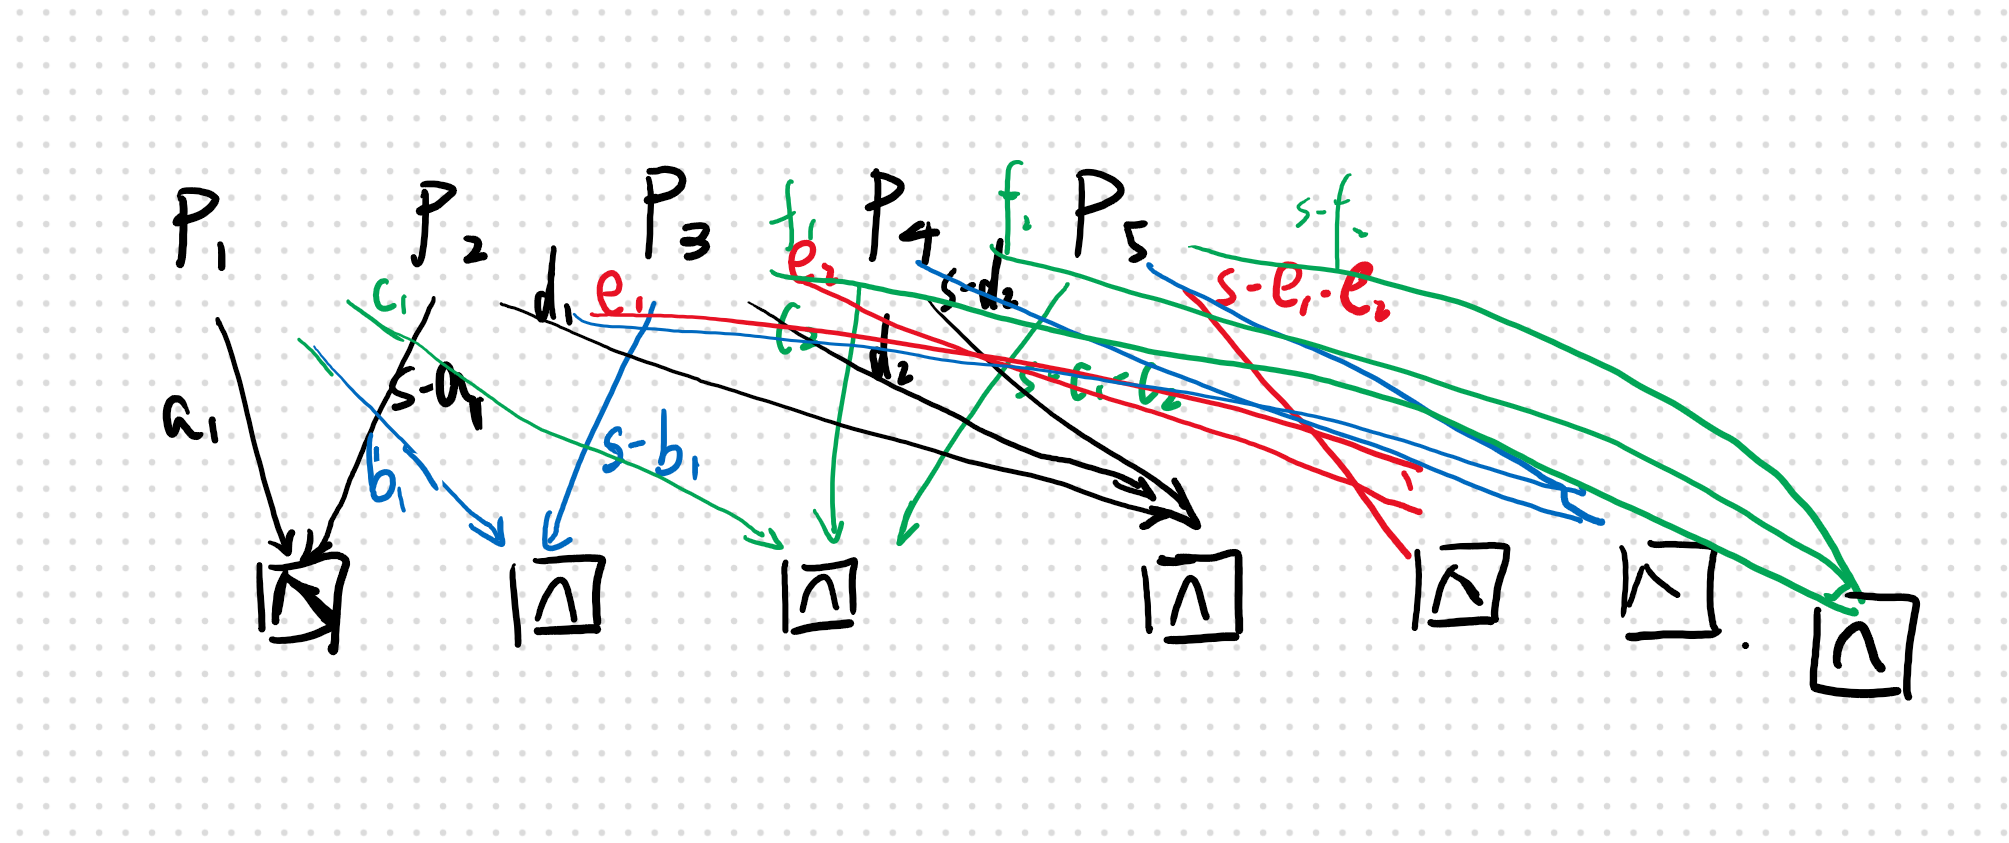
\includegraphics[scale=0.3]{1.png}
                \end{figure}
                \begin{center}
                \begin{tabular}{|c|c|}
                        \hline
                        $p_1$ & $a_1,b_1,c_1$\\
                        \hline
                        $p_2$ & $s-a_1,d_1,e_1,f_1$\\
                        \hline
                        $p_3$ & $s-b_1, d_2, e_2, g_1$\\
                        \hline
                        $p_4$ & $c_2, s-d_1-d_2, f_2,g_2$\\
                        \hline
                        $p_5$ & $s-c_1-c_2, s-e_1-e_2, s-f_1-f_2, s-g_1-g_2$\\
                        \hline
                \end{tabular}    
                \end{center}
        \end{solution*}
        \vspace{20mm}
        \item Let $\rho =\{P_1, P_2, . . . , P_{20}\}$ be a set of $20$ participants.  Let $\tau =\{ A:A \in P,|A|\geq11\}$ be an access structure.
        \begin{enumerate}
                \item If $\tau$ is realized with the monotone circuit construction, how many numbers are there in theshare of each participant?
                \item If $\tau$ is realized with $Shamir’s (11,20)-threshold$ secret sharing scheme, how many numbersare there in the share of each participant?
        \end{enumerate}
        \begin{solution*}
                \leavevmode\\
                \begin{enumerate}
                        \item W.L.O.G. use $P_1$ as example.\\
                        The basis $\tau_0$ of $\tau: \{ A | A \subseteq P, |A| = 11 \}$ \\
                        $p_1$ share is $C_{19}^{10}$
                        \item each participant have only one share $S_i$ for evert $P_i$, So, there is only one number in the share of each participant.
                \end{enumerate}
        \end{solution*}
\end{enumerate}
\end{document}